%!TEX root = foo-thesis.tex

\chapter{Featureberechnung}
\label{chap:feature-calc}

Im Folgenden sollen die wichtigsten Bestandteile der Featureberechnung im \textit{Feature-Extraction}-Ansatz motiviert und erläutert werden. Der vollständige Ablauf des Prozesses, der noch das im nächsten Kapitel behandelte \textit{Uniqueness}-Konzept beinhaltet, findet sich dort in Abbildung \ref{fig:feature_extraction}. Die Featureberechnung ermittelt letztlich für jeden Punkt dessen Featurevektor, der vom Modell zur \textit{Prediction} der Klasse genutzt wird.

\section{Scales}

Um einen Punkt zu charakterisieren, wird seine lokale Nachbarschaft betrachtet. Für die Ermittlung dieser Nachbarschaft gibt es zwei häufig genutzte Wege: die \textit{k} nächsten Nachbarn zu nehmen oder alle Nachbarn, die im vorgegebenen Radius einer Kugel um den Ursprungspunkt liegen. Der Vorteil an den \textit{k} Nachbarn ist, dass man sich über die betrachtete Nachbarzahl sicher sein kann. Allerdings hängt der dabei betrachtete Radius erheblich von der lokalen Punktdichte ab: Beim \textit{Mobile Mapping} etwa wird für Punkte auf der Trajektorie des Laserscannerfahrzeugs mit demselben \textit{k} ein deutlich geringerer Radius betrachtet als für Punkte auf der anderen, nicht befahrenen Straßenseite. Abbildung \ref{fig:knn_vs_scale} stellt dies an zwei Beispielpunkten anschaulich dar. Deshalb eignet sich die Radiusbetrachtung besser für konsistente und über verschiedene Punkte vergleichbare geometrische Features \citep{Thomas.etal-2018}. Diese Art der Nachbarschaftsbetrachtung - von nun an werden die Radii \textit{Scales} genannt - findet in dem \textit{Feature-Extraction}-Ansatz entsprechend Verwendung. \\

\begin{figure}
    \subcaptionbox{Trajektorie, k = 60}{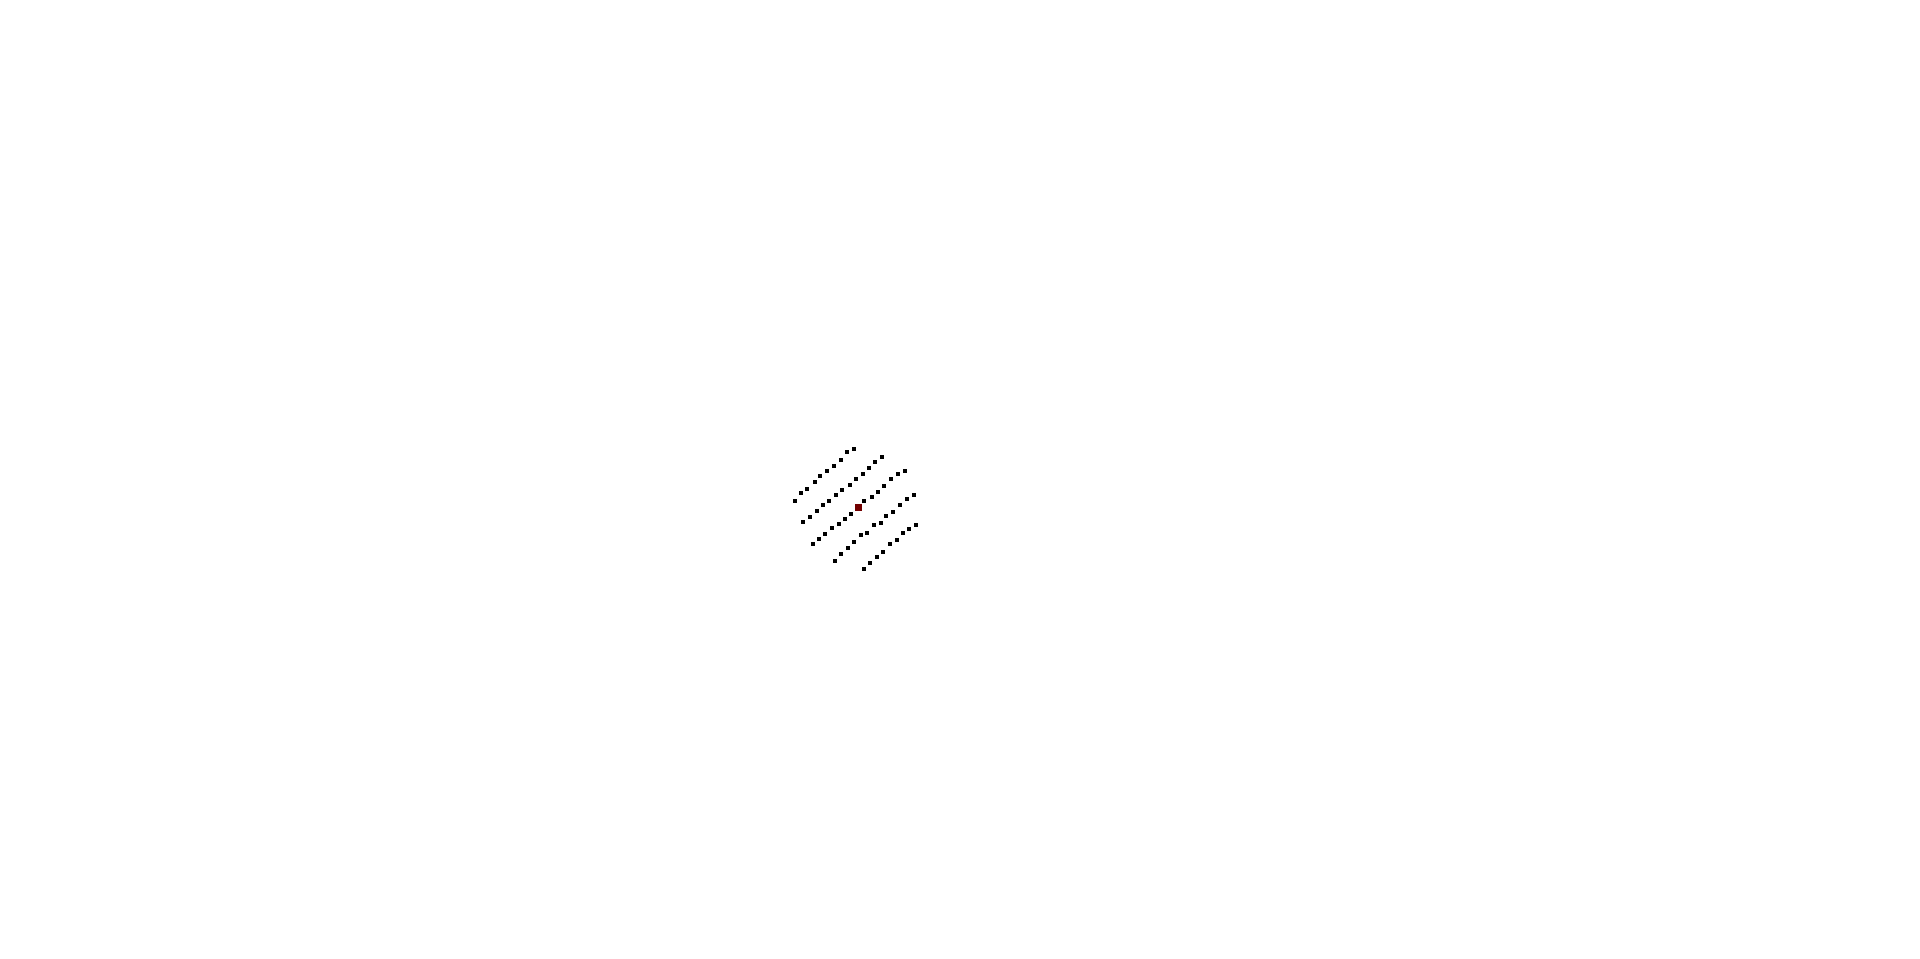
\includegraphics[width=0.5\textwidth]{graphics/traj_knn_adv}}
    \hfill
    \subcaptionbox{Nicht-Trajektorie, k = 60}{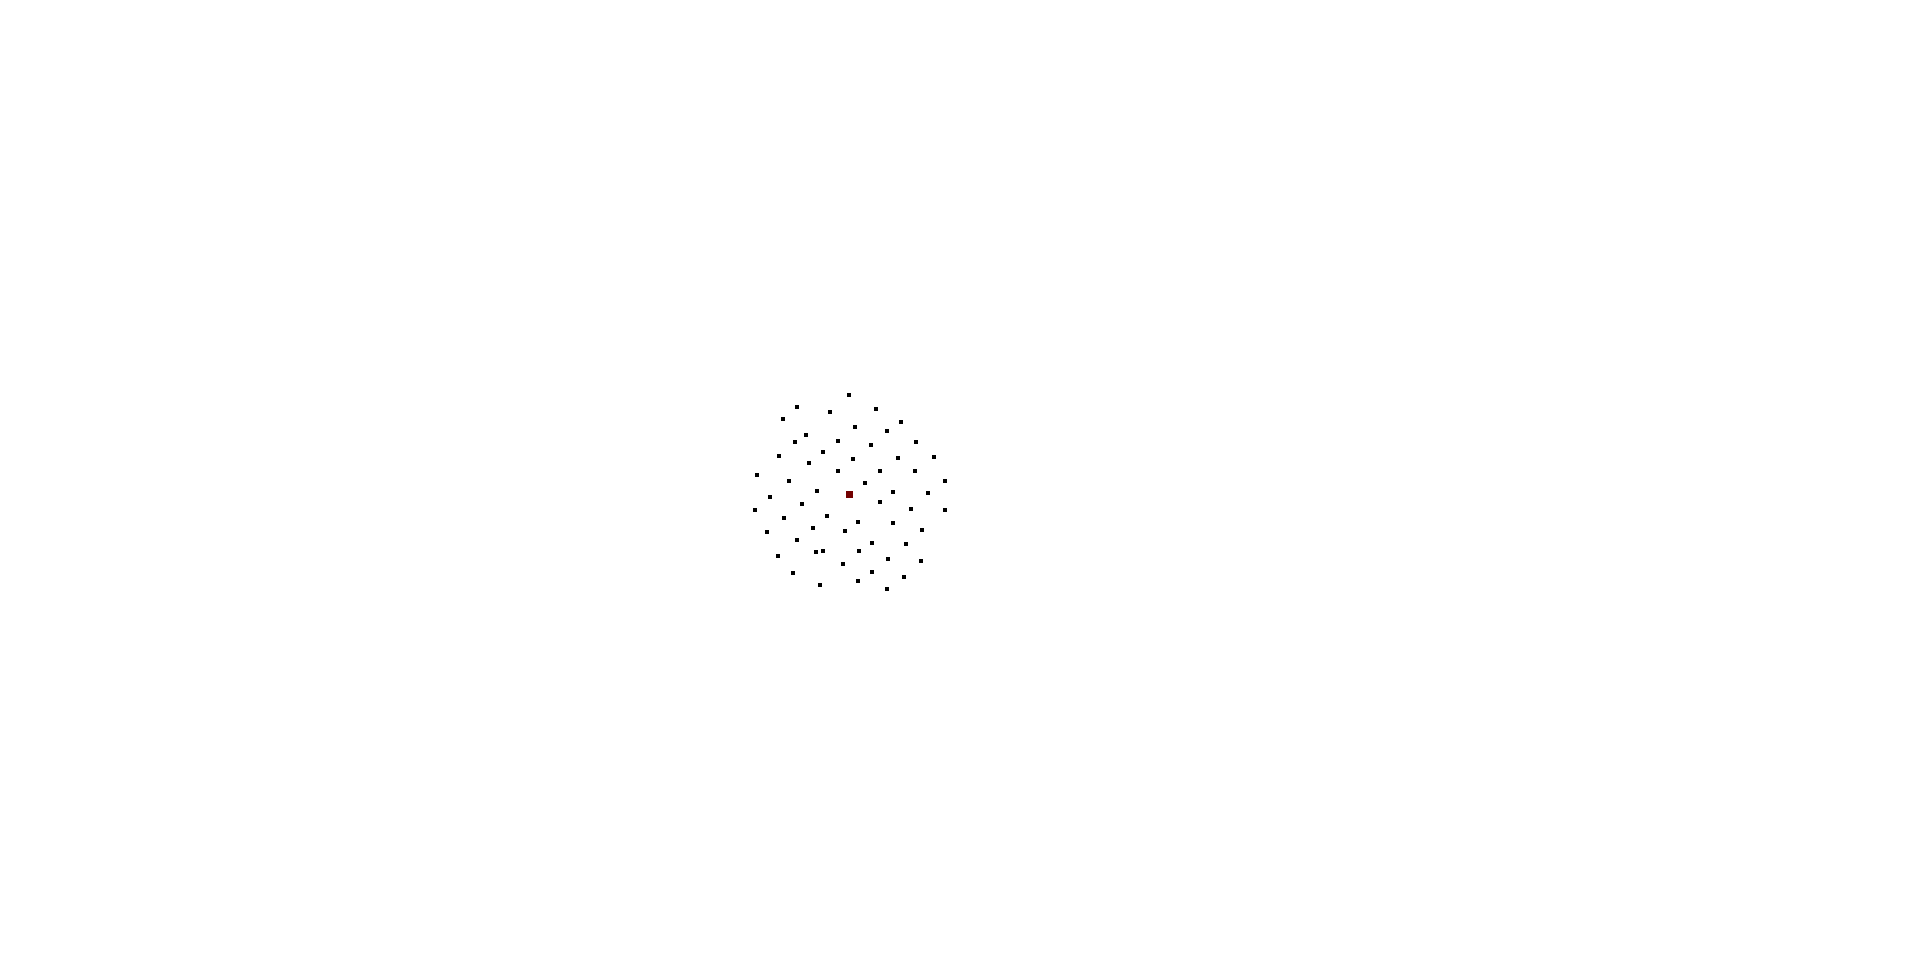
\includegraphics[width=0.5\textwidth]{graphics/nontraj_knn_adv}}
    \par\medskip
    \subcaptionbox{Trajektorie, Radius 10cm}{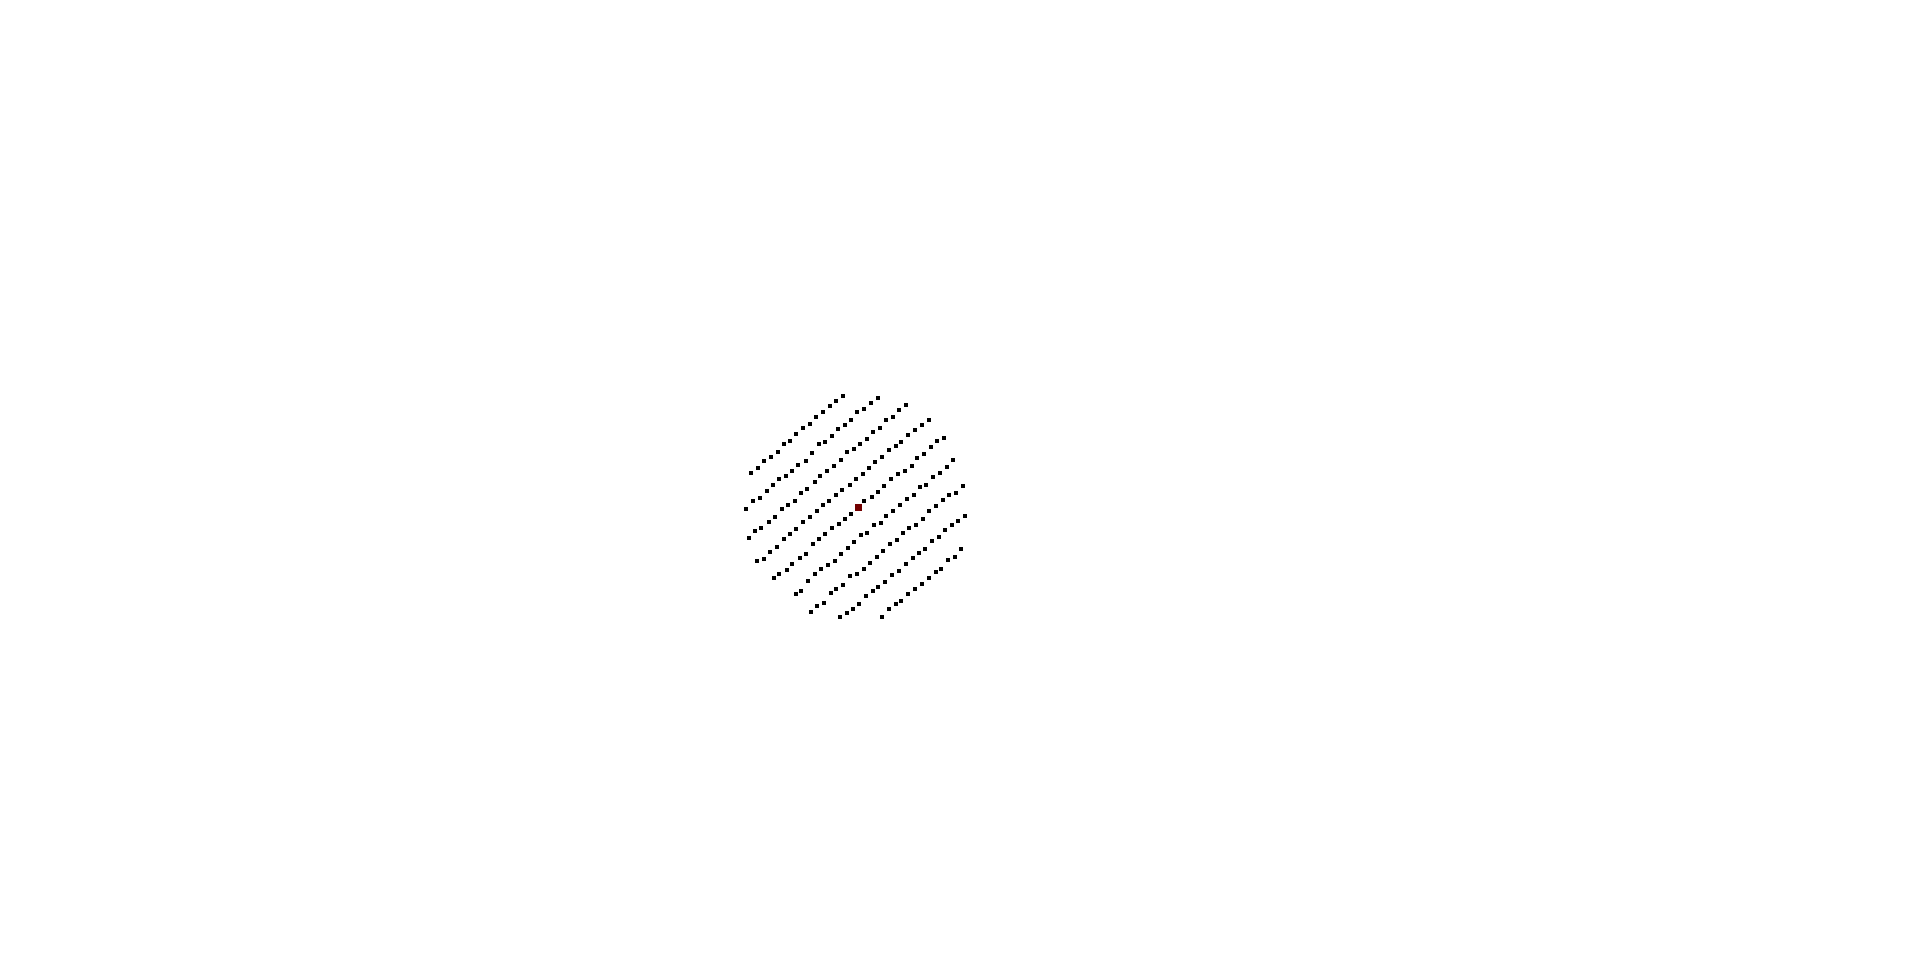
\includegraphics[width=0.5\textwidth]{graphics/traj_scale_adv}}
    \hfill
    \subcaptionbox{Nicht-Trajektorie, Radius 10cm}{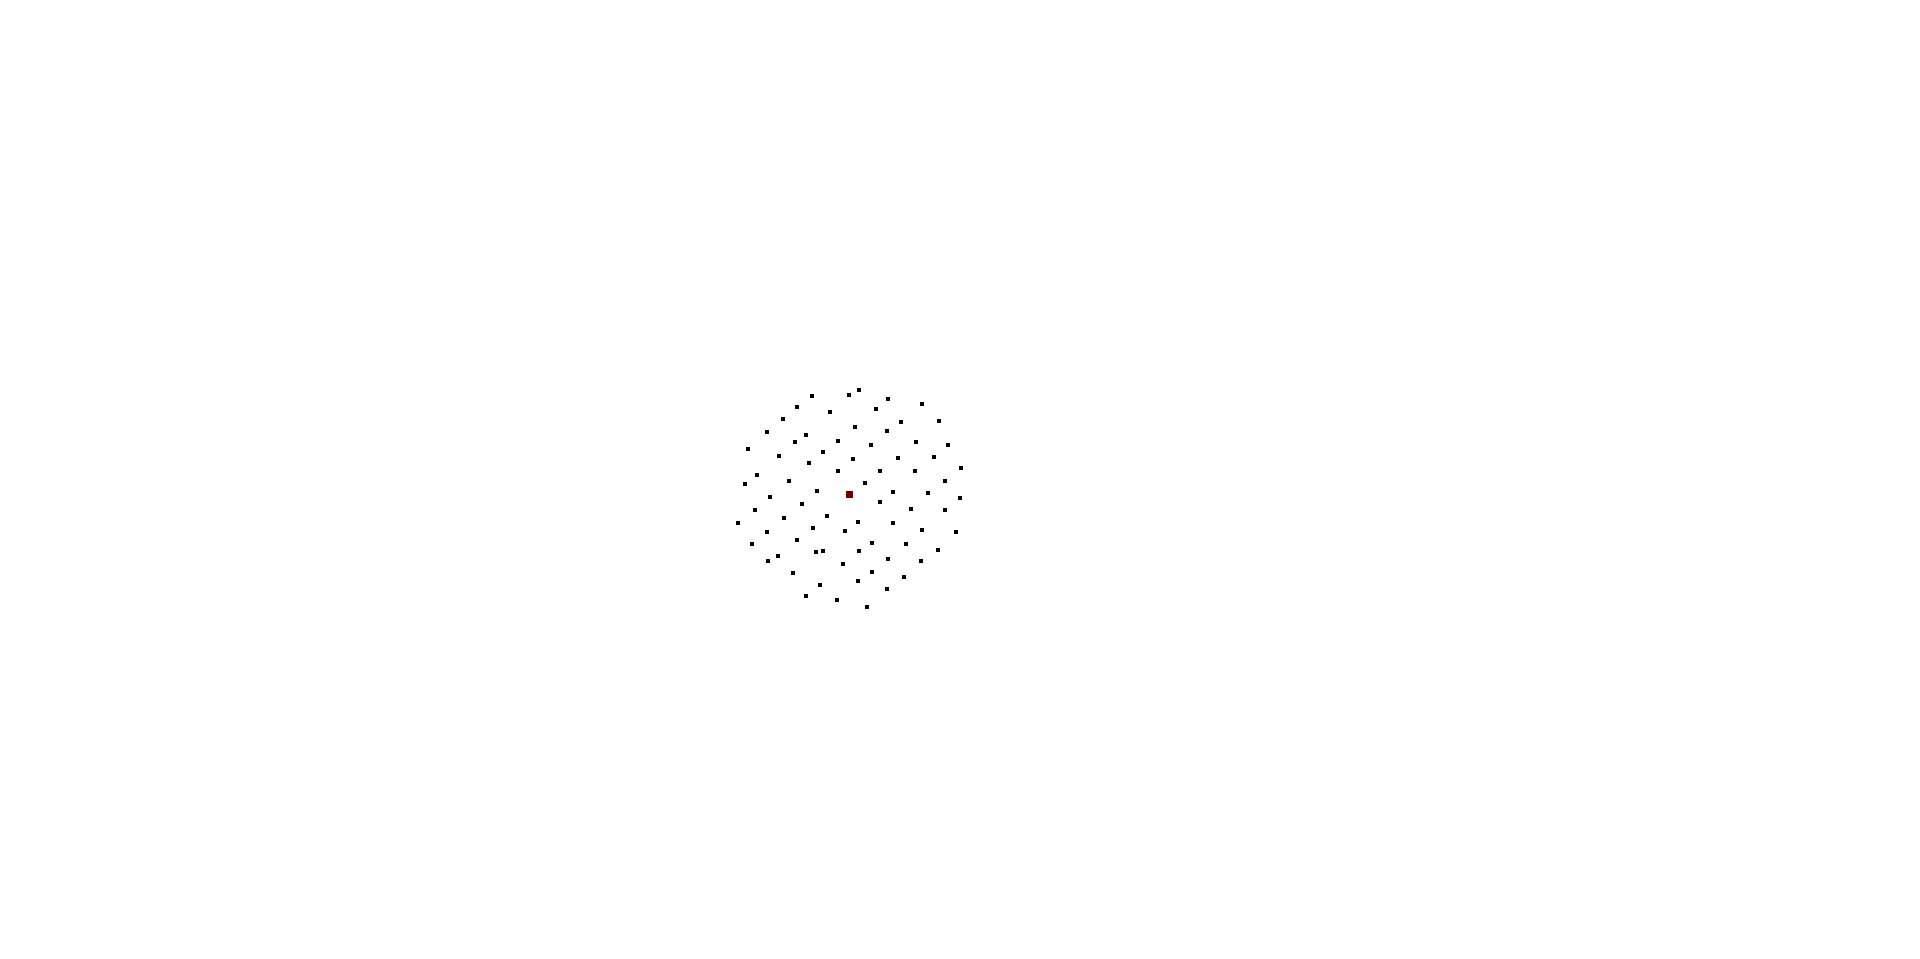
\includegraphics[width=0.5\textwidth]{graphics/nontraj_scale_adv}}
    \caption{Visualisierungen der Nachbarschaften zweier Punkte (zentral, rot gefärbt) auf der Trajektorie bzw. dem restlichen Teil, ermittelt durch die k nächsten Nachbarn bzw. einen festen Radius. Die Bilder sind maßstabsgerecht.}
    \label{fig:knn_vs_scale}
\end{figure}

Um trotz der oftmals Millionen von Punkten einer Punktwolke schnell positionelle Beziehungen herzustellen, wozu etwa das Finden der Nachbarschaft eines Punktes gehört, bedarf es dafür geeigneter Datenstrukturen. Eine solche ist auch der \textit{k-d}-Baum, der einen effizienten Zugriff auf multidimensionale Daten erlaubt, wie es die 3D-Punktkoordinaten sind. Das \texttt{PCTool} sieht dafür die Klasse \texttt{SpatialSearch} vor, die intern einen \textit{k-d}-Baum implementiert und eine einfach zu nutzende Schnittstelle bietet. So können mit jeweils einem Funktionsaufruf sowohl die \textit{k} nächsten Nachbarn einer 3D-Position oder eines Punktindizes gefunden werden als auch alle Nachbarn in einem vorgegebenen Scale. \\\\
Die nächste Frage ist, welche konkreten Scales genutzt werden. Dass überhaupt die Nutzung mehrerer Scales sinnvoll ist, zeigt sich beim Blick auf verschiedene Objekte, die es zu erkennen gilt. Zum einen sind gerade Schlaglöcher häufig unregelmäßige Strukturen, die in vielerlei Ausprägungen vorkommen können: über mehrere Größen hinweg sowie in sehr runden oder eher länglichen Formen. Flickstellen zeichnen sich vorzugsweise in kleinem Scale aus durch ihre hohen Intensitätsunterschiede zu ihrer Umgebung. Bei größeren Gullys wird der innere, mittige Bereich hingegen erst mit deutlich größerem Scale auffällig, da er im kleinen Bereich sehr planar und kaum von der gewöhnlichen Straße zu unterscheiden ist. Um mit diesen verschiedenen Granularitäten umgehen zu können, werden mehrere, an typische Objektgrößen angepasste, Scales genutzt. \\
Um einen Eindruck von den durchschnittlichen Nachbarzahlen verschiedener Scales zu erhalten, sind diese in Tabelle \ref{table:neighbor_counts} (auf Ganzzahlen gerundet) aufgelistet für die Trainingspunktwolke, jeweils auch separat für den Trajektorie- und den restlichen Teil. Den Daten ist Folgendes zu entnehmen:
\begin{itemize}
    \item Für größere Scales steigen die Nachbarzahlen immer stärker an.
    \item Die Nachbarzahlen für Punkte auf der abgeschätzten Trajektorie sind in etwa doppelt so hoch wie für Punkte auf der restlichen Punktwolke. Dies gibt eine weitere Begründung für die in der Straßenextraktion vorgenommene Trennung in einen Trajektorie- und einen restlichen Teil.
    \item Die gesamtheitlichen Zahlen eines Scales liegen näher an denen der Trajektorie. Dies verdeutlicht die Tatsache, dass auf der vom Laserscannerfahrzeug gefahrenen Strecke deutlich mehr Punkte erfasst werden als in der übrigen Umgebung.
\end{itemize}
Laufzeiten für insbesondere die größeren Scales werden in Kapitel \ref{chap:eval} aufgeführt, doch wird hieraus bereits die Beschränkung auf möglichst kleine Scales ersichtlich.

\begin{table}
\centering
\begin{tabular}{c|c|c|c|c|c|c|c|c|c|c}
 & 1$cm$ & 3$cm$ & 6$cm$ & 9$cm$ & 12$cm$ & 15$cm$ & 20$cm$ & 30$cm$ & 40$cm$ & 50$cm$ \\
\hline
Trajektorie & 2 & 15 & 58 & 131 & 232 & 361 & 639 & 1417 & 2480 & 3812 \\
Rest        & 1 &  7 & 28 &  62 & 110 & 171 & 304 &  683 & 1211 & 1887 \\
\hline
\textbf{Gesamt} & \textbf{2} & \textbf{13} & \textbf{48} & \textbf{109} & \textbf{192} & \textbf{299} & \textbf{530} & \textbf{1178} & \textbf{2068} & \textbf{3186} \\
\end{tabular}
\caption{Die durchschnittlichen Nachbarzahlen für ausgewählte Scales, außerdem getrennt aufgeführt für verschiedene Teile der Punktwolke.}
\label{table:neighbor_counts}
\end{table}

Für die unteren Scales wird hier die Grenze bei 3$cm$ angesetzt. Dies ist gering genug für die Feinheiten der Flickstellen oder potenziell sehr kleine Schlaglöcher. Um aussagekräfige Features aus Nachbarschaften zu extrahieren und nicht zu stark von Messungenauigkeiten beeinflusst zu werden, benötigt es eine gewisse Grundanzahl an Nachbarn. Die noch kleineren Scales erfüllen dies - wie der Tabelle zu entnehmen - nicht und werden daher nicht verwendet. Bei den größeren Scales muss abgewogen werden zwischen ihrem zusätzlichen Informationsgehalt und der steigenden Verarbeitungsdauer. Wie bereits erwähnt, sind die großen Scales vor allem sinnvoll für die mittigen Punkte von Gullys. Allerdings genügt auch für diese Punkte ein Scale von etwa 25$cm$, um zu charakteristischen Stellen des Gullys zu reichen wie dem Innenring, weshalb dies die naheliegende obere Schranke darstellt. Da diese Arbeit einen stärkeren Fokus auf die Schadenserkennung legt als auf die vollständige Identifikation von Gullys, liegt der maximale Scale für die standardmäßigen Versuche bei nur 15$cm$. In Kapitel \ref{chap:eval} findet sich auch ein Vergleich zu einem Experiment mit zusätzlichen größeren Scales. In der Spanne von 3$cm$ bis 15$cm$ wird nun jeder Scale im Abstand von wiederum 3$cm$ für die Featureberechnung genutzt. Dies soll einerseits eine angemessene Menge von Scales darstellen, andererseits typische Größen von anzufindenden Schlaglöchern abdecken.

\section{Ein- und mehrwertige Features}

Als Features für Punkte kommen zum einen einwertige Daten in Betracht. Dies umfasst zum Beispiel
\begin{itemize}
    \item Attribute direkt wie die Intensität
    \item Werte, die sich aus der Punktenachbarschaft ergeben, etwa aus der Verteilung der umliegenden 3D-Koordinaten
    \item kumulierte Formen obiger Daten, etwa Durchschnitte oder Standardabweichungen davon
\end{itemize}
Daneben gibt es auch die Möglichkeit für mehrwertige Features. Diese können etwa als Histogramme ausgedrückt werden, also Häufigkeitsverteilungen für bestimmte numerische Merkmale. Sie sind zusammengesetzt aus mehreren sogenannten Bins, welche die Anzahl der Observationen zählen, die in den von ihnen aufgespannten Wertebereich fallen. In dieser Arbeit entspricht eine Observation dem Merkmal eines Punktes, etwa einem Intensitätswert. Die absolute Zahl an Observationen in einem Bin wird \textit{Count} genannt, der entsprechende relative Wert - bezogen auf die Gesamtzahl an Observationen im Histogramm - \textit{Frequency}. Vorteile von Histogrammen sind insbesondere folgende \citep{Rusu.etal-2008}:
\begin{itemize}
    \item Sie besitzen eine grundsätzlich höhere Aussagekraft durch die genauere Charakterisierung der Nachbarschaft. Was sich etwa in einem Durchschnittswert durch entgegengesetzte Größen aufheben würde, kann nun präziser dargestellt werden. Mehr und damit feinere Bins, d.h. jeweils kleinere Wertebereiche, können die Aussagekraft potenziell steigern. Allerdings resultiert dies unter Umständen in einer zu starken Verteilung der Häufigkeiten, sodass charakteristische Ausschläge verloren gehen.
    \item Die oben aufgeführten teilweise erheblichen Unterschiede der Dichte an verschiedenen Stellen einer \textit{Mobile-Mapping}-Punktwolke machen einwertige Features unter Umständen schwierig vergleichbar für einen festen Scale. Bei Histogrammen kann dieses Problem abgeschwächt werden, da durch das Einsortieren in Bins die Werte normalisiert werden in den Bereich von 0 bis 1, und zwar unabhängig von der Anzahl der Nachbarn. Deswegen werden im Ansatz zum Vergleich zwischen Histogrammen und auch für die letztlichen Featurevektoren lediglich die \textit{Frequencies} betrachtet.
    \item Der Umgang mit Außenseiterpunkten (\textit{Outliern}), die teilweise von Messungenauigkeiten stammen, wird erleichtert. Während sie bei einwertigen Features den Wert stark verzerren können - sofern nicht laufzeitintensivere Berechnungen wie der Median durchgeführt werden -, erhöhen sie beim Histogramm nur die \textit{Frequency} eines Bins leicht und sind somit beinahe wie leere Bins zu behandeln. Zwar werden solche \textit{Outlier} bei den Intensitäten im \textit{Preprocessing} möglichst beseitigt. Bei den unnormalisierten 3D-Koordinaten sind sie aber weiterhin möglich und potenziell hinderlich.
    \item Histogramme sind, im Gegensatz zu einigen anderen lokalen Deskriptoren \citep{Han.etal-2018}, unabhängig von Transformationen der Punktwolke wie Rotation oder Translation.
\end{itemize}
Für diesen Ansatz sollen lediglich mehrwertige Features eingesetzt werden. Ein Vergleich mit der Nutzung nur einwertiger Features findet sich in Kapitel \ref{chap:eval}.
Im Zuge dieser Arbeit wurde im \texttt{PCTool} eine eigene Histogramm-Datenstruktur implementiert. Das geschah zum einen aus Mangel an Alternativen, zum anderen, um für den \textit{Feature-Extraction}-Ansatz nötige Methoden wie ein Distanzmaß oder die Berechnung einer durchschnittlichen Repräsentation (siehe Kapitel \ref{chap:uniqueness}) direkt einzubauen. Ansonsten werden gewöhnliche Funktionalitäten bereitgestellt wie das Füllen der Bins mit gegebenen Daten sowie die Rückgabe der ermittelten \textit{Frequencies}. \\
Zum Zwecke der Erweiterbarkeit und optimierter Speichernutzung ist \texttt{Histogram} eine abstrakte Klasse, die nur die Counts speichert. Ein Histogramm kann linear oder nicht-linear sein, je nachdem, ob dessen Bins einen kontinuierlichen und gleichmäßig aufgeteilten Wertebereich aufspannen. Diese Arten werden in den beiden Unterklassen \texttt{LinearHistogram} und \texttt{NonLinearHistogram} umgesetzt mit ihren entsprechenden internen Arbeitsweisen. In diesem Ansatz wurden keine nicht-linearen Histogramme genutzt, was insbesondere an ihrer verhältnismäßig aufwändigen Berechnung liegt: Statt die Bins direkt in einer Iteration der Daten zu befüllen, ist eine vorherige Sortierung letzterer nötig. In Verbindung mit größeren Scales macht sich diese $nlogn$-Komplexität in der Laufzeit bemerkbar. Ein Vorteil der Nutzung nicht-linearer Histogramme könnte aber darin liegen, genauere Kontrolle über die Wertebereiche zu haben, wenn etwa bekannt ist, dass in bestimmten Größenordnungen keine Werte zu erwarten sind. \\ 
Die dritte Unterklasse ist das \texttt{AbsoluteHistogram}. Dieses speichert mehrere (grundsätzlich unabhängige) einwertige Features anstatt echter Bins, die als die \textit{Frequencies} betrachtet werden. Da also keine \textit{Counts} existieren, handelt es sich der grundlegenden Bedeutung nach um kein Histogramm. Die \textit{Frequencies} ergeben summiert auch nicht 1, wobei die im Experiment genutzten einwertigen Features jeweils zwischen 0 und 1 liegen. Es ist vornehmlich eingeführt worden für den einheitlichen Umgang mit ein- und mehrwertigen Features bezüglich der Speicherung und des Distanzmaßes, obwohl die Semantik eine andere ist. \\\\
Wenn in Abschnitten des Wertebereichs kaum Werte tatsächlich vorkommen, hat dies bei linearen Histogramme teilweise viele leere Bins zur Folge, d.h. Bins mit einem \textit{Count} und demzufolge einer \textit{Frequency} von 0. Um während der Featureberechnung und der Zwischenspeicherung aller Featurevektoren etwas Speicher zu sparen, werden solche Folgen von leeren Bins verkürzt abgespeichert: Statt $k$ ($k \geq 2$) konsekutiver $0.0$-Einträge wird ein Paar geschrieben aus Erkennungssymbol für diese Verkürzung (etwa \texttt{infinity}) und dem $k$ selbst. Beim abschließenden Schreiben der Featurevektoren können diese wieder leicht in ihre ursprüngliche Größe überführt werden. Um ferner etwas Rauschen zu reduzieren, der zum Beispiel durch einen \textit{Outlier} verursacht wurde, wird ein Schwellwert von $0.005$ genutzt statt des festen Werts von $0.0$, damit ein Bin als leer gilt. Zwar sorgt dies dafür, dass die Summe aller \textit{Frequencies} eines Histogramms im Featurevektor nicht mehr unbedingt gleich 1 ist; dies führte allerdings zu keinen signifikanten Änderungen der \textit{Predictions}. \\
Da die von den Histogrammen aufgespannten Wertebereiche nicht immer die theoretisch möglichen Wertebereiche vollständig abdecken, gilt außerdem: Werte, die kleiner als die Werte im ersten Bin sind, und Werte, die größer als die Werte im letzten Bin sind, werden entsprechend dem ersten bzw. letzten Bin zugerechnet. Auf diese Weise werden immer alle Werte der Nachbarschaft berücksichtigt. \\
Als \textit{Featureraum} sollen künftig einzelne lineare oder absolute Histogramme bezeichnet werden, etwa der Featureraum der Intensität. Pro Scale und Punkt werden mehrere solcher Featureräume berechnet; alle Featureräume aller Scales bilden schließlich den Featurevektor pro Punkt, der für die \textit{Prediction} seiner Klasse genutzt wird.

\section{Approximation für größere Scales}

Die Zahl der Nachbarn eines Punktes erhöht sich mit linear steigendem Scale deutlich stärker als linear. Entsprechend verlängert sich auch die Prozessierungsdauer pro Scale erheblich. Da unter Umständen solche größeren Scales aber nicht einfach ausgelassen werden können, beinhaltet der eigene Ansatz die Möglichkeit einer Approximation der Featurevektoren auf Basis reduzierter Originaldaten. Die Motivation dahinter ist, dass für feine Stellen die kleinen Scales gedacht sind, die tatsächlich jeden Punkt berücksichtigen. Im größeren Scale genügt eine regelmäßig abgetastete Teilmenge aller Punkte.  \\
Zu diesem Zweck wird, noch vor der Extraktion der Features, eine Dichtereduktion auf der Punktwolke ausgeführt. Diese Operation kann die Punktmenge senken, indem alle Punkte etwa innerhalb eines Würfels zu einem einzigen Punkt zusammengefasst werden. Dazu wird intern eine Kopie der originalen Punktwolke angelegt, die sogenannte \textit{Half Edge Length} bestimmt, welche die Stärke der Dichtereduktion festlegt, und letztere entsprechend vorgenommen. Auf dieser reduzierten Punktwolke werden nun ebenfalls ein \textit{k-d}-Baum für den effizienten Zugriff erzeugt sowie die Features auf analoge Weise berechnet. Der Schwellwert für die Ausführung der Operation liegt bei 20$cm$. Für kleinere Scales ist der Mehraufwand aus Kopie, der Dichtereduktion und der gleich erklärten Approximation zu groß im Vergleich zur standardmäßigen Prozessierungszeit ohne Dichtereduktion. \\\\
Die Dichtereduktion verringert effektiv die Nachbarzahl jedes Punktes und somit insbesondere die Dauer der Featureberechnung. Allerdings sind anschließend nur Features berechnet worden für eine Teilmenge der ursprünglichen Punkte. Da für jeden Punkt ein vollständiger Featurevektor erwartet wird für die letztliche \textit{Prediction}, muss dieser jeweils aus den bisher ermittelten approximiert werden. Der Ansatz ist hierbei der folgende: Für jeden Originalpunkt $P$ wird dessen Nachbarschaft $\mathfrak{N}$ in der reduzierten Punktwolke bestimmt. Der Scale für die Suche beträgt 3$cm$, um keine zu weit entfernten Punkte und somit Featurevektoren einzubeziehen. Für den Ausnahmefall, dass sich kein einziger Punkt in diesem Scale befindet, wird lediglich der nächste Punkt (\textit{kNN} = 1) herangezogen. Da nähere Punkte eher den tatsächlichen Featurevektor von $P$ für diesen Scale repräsentieren, sollen sie auch stärker bei der Approximation gewichtet werden. Dies geschieht über die inverse Distanz zu $P$, wobei dieser Wert noch durch die Summe aller inversen Distanzen normalisiert wird:
\begin{equation}
    \omega_i = \nicefrac{\frac{1}{d(P, \mathfrak{N}_i)}}{\sum_{j = 1}^{|\mathfrak{N}|}{\frac{1}{d(P, \mathfrak{N}_j)}}}, i \in \{1, ..., |\mathfrak{N}|\}
\end{equation}
Dabei entspricht $d$ der Distanzfunktion im euklidischen Raum. Mithilfe der Gewichtungen und der Featurevektoren $\mathfrak{F}$ der Nachbarschaft kann schließlich der Featurevektor $F$ von $P$ als gewichteter Durchschnitt berechnet werden \citep{Rusu.etal-2009}, umgesetzt durch die \texttt{weightedMean}-Methode der \texttt{Histogram}-Klasse:
\begin{equation}
    F_P = \sum\limits_{i = 1}^{|\mathfrak{N}|}{\omega_i * \mathfrak{F}_{\mathfrak{N}_i}}
\end{equation}
Dieser Approximationsschritt soll also die Prozessierungszeit senken und die einzelnen Featurevektoren dabei trotzdem hinreichend genau darstellen. Ein Vergleich der Zeitersparnis durch Nutzung der Approximation für größere Scales findet sich in Kapitel \ref{chap:eval}.

\section{Genutzte Features}

Die genutzten Features sollen Unterscheidungsmerkmale zwischen den verschiedenen Klassen ausdrücken. Sie basieren auf den in der Punktwolke gespeicherten Intensitätswerten sowie 3D-Koordinaten. Alle Features werden durch Histogramme repräsentiert, wobei jedes dieser aus 12 Bins besteht. Dieser Wert soll einen Ausgleich schaffen zwischen einem ausreichenden Detailgrad und zu großer Streuung der \textit{Frequencies}.

\subsection*{Intensitätsbasiert}

Die reine Intensität hebt bereits Fahrbahnmarkierungen durch einen sehr hohen und Ölflecken durch einen sehr niedrigen Wert hervor. Zhiqiang \textit{et al.} \cite{Zhiqiang.etal-2019} nutzen dieses Attribut ebenfalls als Teil ihrer Featurevektoren, wobei dort noch eine Interpolation über Gewichtungen invers zur Distanz vorgenommen wird. Es gibt einzelne Punkte mit extremen Ausschlägen, die weder zur einen noch zur anderen Klasse gehören, siehe Abbildung \ref{fig:fake_road_marking}. Mit dem Ziel, solche Außenseiter auch entsprechend zu klassifizieren, wird ein Histogramm gebildet der umliegenden Intensitäten. Dessen Wertebereich von 0,2 bis 0,8 bildet dabei ungefähr das Spektrum der häufig vorkommenden Intensitäten ab, mit den Ölflecken durchschnittlich knapp unter 0,2 und den Fahrbahnmarkierungen knapp über 0,8. Für die erwähnten Außenseiter könnte dieses mehrwertige Feature im kleinen Scale ähnlich dem von Fahrbahnmarkierungen sein, was sich im größeren Scale jedoch wieder ausgleicht und die Punkte voneinander abgrenzt. Auch Schlaglöcher haben oft, bedingt durch den abgetragenen Asphalt, eine geringere Intensität als ihre unmittelbare Umgebung. \\
Das nächste Feature umfasst die lokalen Intensitätsunterschiede der Nachbarn zum jeweiligen Ursprungspunkt. Neben Fahrbahnmarkierungen und Ölflecken sind gerade Flickstellen dadurch gekennzeichnet, dass die deutlich dunklere Fugendichtmasse, die Streifen mit wenigen Zentimetern Breite bildet, sich abhebt vom Rest der umliegenden Oberfläche und somit die meist rechteckige Form erkennen lässt. Diese Differenzen sollen dabei helfen, in ihrer Intensität auffällige Stellen einzugrenzen und zu erkennen. Dazu wird ein Histogramm erstellt aus den absoluten Differenzen der Intensitäten mit einem Wertebereich von 0 bis 0,3. Die Obergrenze schließt bereits - trotz theoretischem Maximalwert von 1 - den größten Teil der tatsächlich vorkommenden Differenzen ein, darunter diejenigen zwischen Flickstellen und angrenzender gewöhnlicher Straße. \\
Zusammengenommen charakterisieren die beiden Histogramme die Intensität eines Punktes und wie sehr sie sich unterscheidet von dessen Nachbarschaft.

\begin{figure}[!ht]
    \centering
    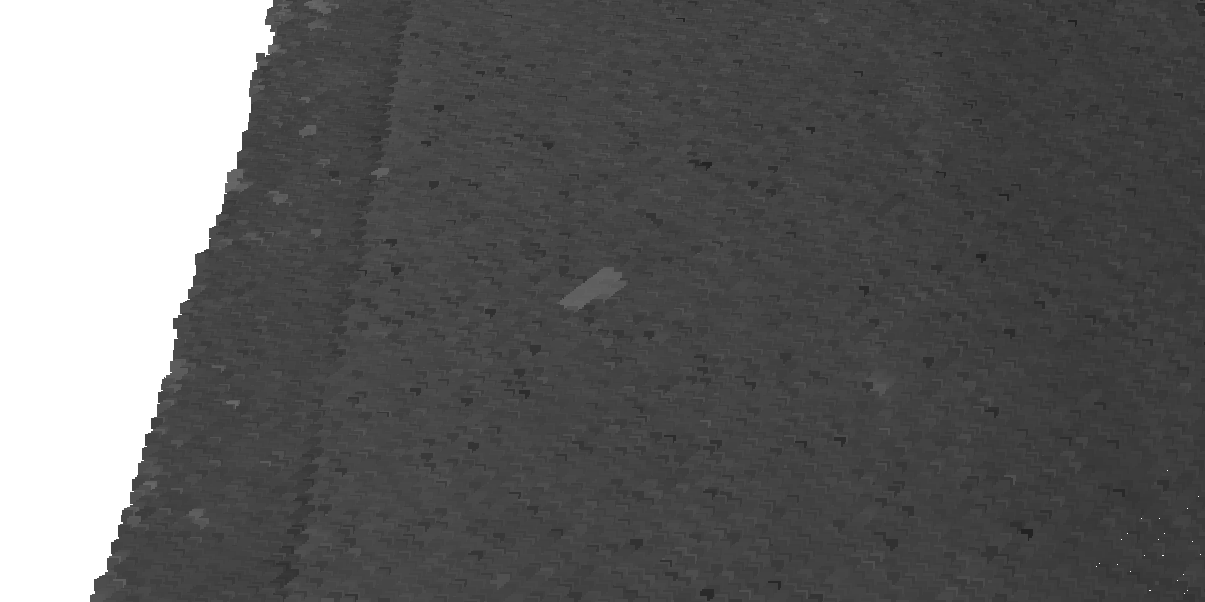
\includegraphics[width=0.3\textwidth]{graphics/fake_road_marking}
    \caption{Eine kleine Stelle auf der Straße, die eine ähnlich hohe Intensität wie Fahrbahnmarkierungen besitzt.}
    \label{fig:fake_road_marking}
\end{figure}

\subsection*{Koordinatenbasiert}

Es existieren verschiedene Maße, die für einen einzelnen Punkt die Form und Oberfläche seiner lokalen Nachbarschaft beschreiben \citep{Han.etal-2018}. Eine Auswahl dieser grundsätzlich einwertigen Features soll im Folgenden erläutert werden. \\
Die Basis jener Maße ist die Betrachtung der umgebenden 3D-Koordinaten eines Punktes und deren Verteilung. Dies wird repräsentiert durch die Kovarianzmatrix. Grundsätzlich beschreibt die Kovarianz zwischen zwei Variablen einen Grad ihres linearen Zusammenhangs: Ihr Vorzeichen deutet an, ob höhere Werte der einen Variable eher mit höheren oder niedrigeren Werten der anderen Variable einhergehen und umgekehrt. Im konkreten Fall von 3D-Daten sind die Variablen die drei Dimensionen \textit{X}, \textit{Y} und \textit{Z} selbst, die zusammen eine \textit{3×3}-Kovarianzmatrix einer Punktmenge bilden und in ihren Einträgen die Kovarianz zwischen den entsprechenden Dimensionen beschreibt. Die Durchschnitte der Variablen für die Zentrierung der Koordinaten sind hier die Koordinaten des durchschnittlichen Punkts der Menge, dem sogenannten \textit{Centroid}. \\
Ist diese Matrix für einen Punkt und seine Nachbarschaft einmal berechnet, müssen aussagekräfige Informationen daraus extrahiert werden. Für die genutzten Maße geschieht das mittels der drei Eigenwerte der Matrix. Diese bemessen die höchsten Varianzen entlang paarweise orthogonaler Achsen. Die Eigenwerte $\lambda_1$, $\lambda_2$ und $\lambda_3$ werden absteigend sortiert, sodass $\lambda_1 \geq \lambda_2 \geq \lambda_3$. Anschließend werden sie normalisiert durch Division ihrer Gesamtsumme: 
\begin{equation}
    \label{formula:eigen_normalization}
    e_i = \frac{\lambda_i}{\lambda_1 + \lambda_2 + \lambda_3}, i \in \{1, 2, 3\}.
\end{equation}
Die Berechnung der Eigenwerte ist aufwändiger als die der intensitätsbasierten Features. Zu diesem Zweck wurde der \texttt{EigenvalueCalculator} im \texttt{PCTool} implementiert. Dieser baut zu großem Teil auf dem zuvor existierenden \texttt{NormalsEstimator} auf, welcher für alle Punkte parallel ihre abgeschätzte Normale berechnet, die senkrecht auf der approximierten Oberfläche steht. Diese Normale ergibt sich als der Eigenvektor der Kovarianzmatrix mit dem kleinsten Eigenwert. Da in diesem Schritt also die Eigenwerte ohnehin berechnet werden, soll im \texttt{EigenvalueCalculator} beides kombiniert werden. Mit einstellbarem Scale werden die Normalen berechnet und jeweils drei Eigenwerte für alle Punkte zurückgegeben. Daraufhin werden diese entsprechend \ref{formula:eigen_normalization} normalisiert durch Division der Gesamtsumme. \\\\
Mittels der drei normalisierten Eigenwerte können nun die Maße \textit{Linearity}, \textit{Planarity}, \textit{Scattering} (auch \textit{Spherity}) sowie \textit{Local Curvature} (auch \textit{Change of Curvature}, folgend nur \textit{Curvature}) einfach berechnet werden, wie es in Tabelle \ref{table:eigenvalue_features} dargestellt ist. Diese Features werden unter anderem von \cite{Zaboli.etal-2019} und \cite{Li.Cheng-2018} genutzt, um städtische Objekte in \textit{Mobile-Mapping}-Punktwolken zu erkennen. Sie beschreiben, wie linear, eben oder rund die Nachbarschaft eines Punktes sich verhält und wie stark sie sich im Vergleich zu einer Ebene krümmt. Von ihrer Aussagekraft sind sie vergleichbar mit den in \cite{Zhiqiang.etal-2019} genutzten Features \textit{Roughness Index} und \textit{Gaussian Curvature}. Die Berechnung der Maße pro Punkt wird durchgeführt von Objekten der jeweils zuständigen Klasse (\texttt{CurvatureCollector} für \textit{Curvature}, usw.). \\

\begin{table}
\centering
\begin{tabular}{c|c|c|c}
Linearity & Planarity & Scattering & Curvature \\ 
$\frac{e_1 - e_2}{e_1}$ & $\frac{e_2 - e_3}{e_1}$ & $\frac{e_3}{e_1}$ & $\frac{e_3}{e_1 + e_2 + e_3}$ \\
\end{tabular}
\caption{Vier einwertige, auf den Eigenwerten der Kovarianzmatrix basierenden Features zur Beschreibung der Form der lokalen Nachbarschaft.}
\label{table:eigenvalue_features}
\end{table}

Auf Basis dieser einwertigen Features werden dann mehrwertige in Form von Histogrammen gebildet. Dabei hat sich jedoch herausgestellt, dass \textit{Linearity} und \textit{Planarity} nur einen geringen Informationswert bieten bezüglich der Unterscheidungskraft. Deshalb sind diese beiden Maße nicht Teil der koordinatenbasierten Features, sondern lediglich \textit{Scattering} und \textit{Curvature}. Im Experiment mit nur einwertigen Features werden alle vier Werte an die Featurevektoren angehängt. \\
Die Grenzen der Histogramm-Wertebereiche sind zusätzlich vom Scale abhängig, da die Varianz der Werte im kleinen Scale generell höher ist. So können im Radius von wenigen Zentimetern kleine Unterschiede der Koordinaten einen großen Einfluss auf den Wert haben, was auch an der geringen Zahl an Nachbarn liegt (siehe Tabelle \ref{table:neighbor_counts}). Für Scales von 10, 20 und mehr Zentimetern gleicht sich dies für die allermeisten Punkte wieder aus und die Werte nähern sich dem Durchschnitt der gesamten Punktwolke an. Beispielsweise ist der durchschnittliche Wert für \textit{Scattering} in der Trainingspunktwolke im Scale von 3$cm$ gleich 0,013, im Scale von 15$cm$ nur noch 0,001. Dabei ist der \textit{Scattering}-Wert für die hier behandelten Objektklassen ebenso wie die \textit{Curvature} grundsätzlich eher gering und weit entfernt vom maximalen Wert 1. Daher wird jeweils die Obergrenze des Histogramms - die durch manuelle Inspektion für eine gute Unterscheidung zwischen den Klassen festgelegt wurde - angepasst, was in Tabelle \ref{table:eigenvalue_features_impl} für die einzelnen Scales aufgeführt ist.

\begin{table}
\centering
\begin{tabular}{c|c|c|c|c|c}
& 3$cm$ & 6$cm$ & 9$cm$ & 12$cm$ & 15$cm$ \\
\hline
Scattering & 0,05 & 0,02 & 0,01 & 0,005 & 0,005 \\
Curvature  & 0,03 & 0,01 & 0,005 & 0,0025 & 0,0025 \\
\end{tabular}
\caption{Die Obergrenzen der linearen Histogramme von den genutzten Eigenwert-basierten Features für jeden Scale.}
\label{table:eigenvalue_features_impl}
\end{table}

In diesem Ansatz werden keine globalen Features verwendet, die jeweils die gesamte Punktwolke verarbeiten. Während etwa in \cite{Zhiqiang.etal-2019} \textit{Triangulated Irregular Networks} und Verfahren der \textit{Object Segmentation} genutzt werden, um die Umrisse von Objekten wie Schlaglöchern und Rissen zu detektieren, sollen hier nur lokale - also jeweils auf einen Scale beschränkte - Features Anwendung finden.